%%
%% This is file `test-spacing.tex',
%% generated with the docstrip utility.
%%
%% The original source files were:
%%
%% phd.dtx  (with options: `test-spacing')
%% ----------------------------------------------------------------
%% phd --- A package to beautify documents.
%% E-mail: yannislaz@gmail.com
%% Released under the LaTeX Project Public License v1.3c or later
%% See http://www.latex-project.org/lppl.txt
%% ----------------------------------------------------------------
%% 
\documentclass{ltxdoc}
\usepackage[a4paper,left=2.25cm,right=2.25cm,top=2.5cm,
            bottom=2.5cm]{geometry}
\usepackage{phd}

\cxset{style13/.style={
 name=CHAPTER,
 chapter toc=true,
 chapter spaceout = none,
 chapter numbering=arabic,
 chapter after={\vskip0pt\par},
 number font-size= HUGE,
 number font-family= sffamily,
 number font-weight= bfseries,
 title font-shape= upshape,
 number color= gray!50,
 number before=\par\vspace*{5pt}\hfill\hfill,
 number dot=,
 number after={\hspace*{7pt}\par},
 number position=rightname,
 chapter font-family= sffamily,
 chapter font-weight= bold,
 chapter font-size= LARGE,
 chapter before={\thinrule\vspace*{20pt}\par\hfill\hfill},
 chapter color= black!50,
 title beforeskip={\vspace*{10pt}},
 title afterskip={\vspace*{50pt}\par},
 title before={\hfill\hfill\raggedleft},
 title after=\par\thinrule,
 title font-family= sffamily,
 title font-color= teal,
 title font-weight= bfseries,
 title font-size= huge,
 section indent=-1em,
 section align= left,
 section numbering= arabic,
 section indent=0pt,
 section beforeskip=0pt,
 section afterskip= 10pt,
 section color=teal,
 subsection align= ,
 subsection font-family= sffamily,
 subsection font-weight= bfseries,
 subsection color = teal,
 subsection font-size= large,
 subsection font-shape=,
 subparagraph number after=,
 subsubsection align=,
 blank page text=,
 chapter opening=any,
}
}

\usepackage{lipsum}
\begin{document}
\cxset{style13}
\chapter{Petri Dishes Library}

The package defines a style for drawing places of Petri nets. 

\begin{stylekey}{/tikz/place}
  This style indicates that a node is a place of a Petri net. Usually,
  the text of the node should be empty since places do not contain any
  text. You should use the |label| option to add text outside the node
  like its name or its capacity. You should use the |tokens| options,
  explained in Section~\ref{section-tokens}, to add tokens inside the
  place.
  
\begin{codeexample}[]
\begin{tikzpicture}
  \node[place,label=above:$p_1$,tokens=2]        (p1) {};
  \node[place,label=below:$p_2\ge1$,right=of p1] (p2) {};
\end{tikzpicture}
\end{codeexample}
  
  \begin{stylekey}{/tikz/every place}
    This stype is envoked by the style |place|. To change the
    appearance of places, you can change this style.
\begin{codeexample}[]
\begin{tikzpicture}
  [every place/.style={draw=blue,fill=blue!20,thick,minimum size=9mm}]
  \node[place,tokens=7,label=above:$p_1$]  (p1) {};
  \node[place,structured tokens={3,2,9},
        label=below:$p_2\ge1$,right=of p1] (p2) {};
\end{tikzpicture}
\end{codeexample}
  \end{stylekey}
\end{stylekey}
\cxset{chapter opening=any}
<<<<<<< HEAD
%%%%%%%%%%%%%%%%%%%%%%%%%%%%%%%%%%%%%%%%%%%
%%%%%%  STYLE 10
%%%%%%%%%%%%%%%%%%%%%%%%%%%%%%%%%%%%%%%%%%%

\cxset{
 name=CHAPTER,
 numbering=WORDS,
 number font-size=\huge,
 number font-family=\sffamily,
 number font-weight=\bfseries,
 number before=,
 number dot=,
 number after=\hspace{1em},
 number position=rightname,
 chapter font-family=\sffamily,
 chapter font-weight=\bfseries,
 chapter font-size=\huge,
 chapter before={\vspace*{0.4\textheight}\hfill},
 chapter after={\hfill\hfill\vskip0pt\thinrule\par},
 chapter color={black!90},
 number color=\color{black!90},
 title beforeskip={\vspace*{30pt}},
 title afterskip={\vspace*{30pt}\par},
 title before={\hfill},
 title after={\hfill\hfill},
 title font-family=\sffamily,
 title font-color=\color{black!90},
 title font-weight=\bfseries,
 title font-size=\huge,
 section font-size=\LARGE,
 section font-weight=\normalfont,
 section font-family=\sffamily,
 section align=,
 section numbering=none,
 section indent=-1em,
 section align=\centering,
 section beforeskip=20pt,
 section afterskip=10pt,
 section spaceout=soul,
 section font-shape=,
}

 %set the sectioning commands


\renewsection

\chapter{INTRODUCTION TO STYLE TEN}

\section{Basic Description:}
This chapter style has the unique characteristic that the chapter number is spelled out, rather than being in arabic numerals. The setting for this is the option \lstinline{numeric=WORDS}. Use either a capital for uppercase or \lstinline{numeric=words} for lowercase number labels.

\medskip
\begin{figure}[ht]
\centering
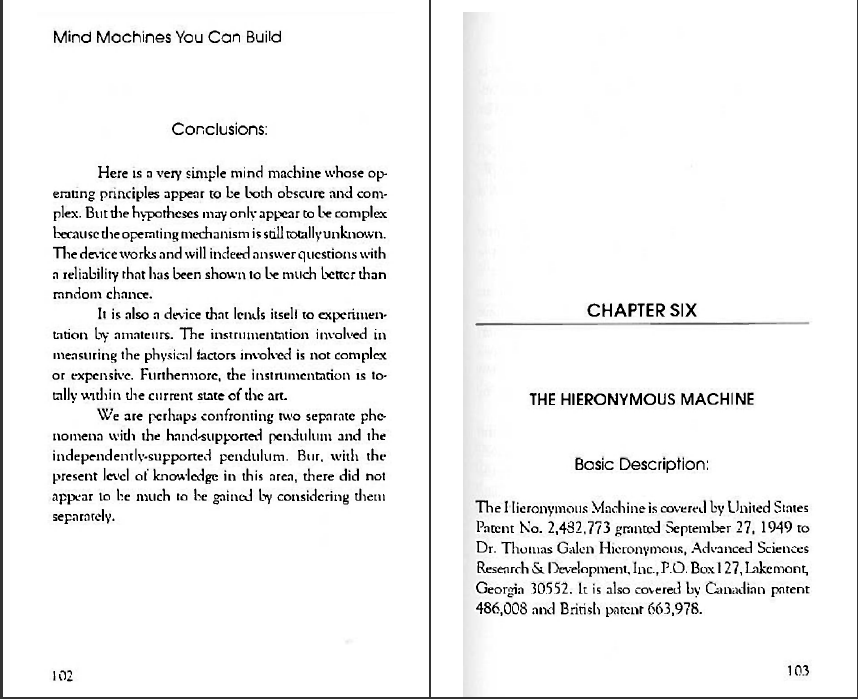
\includegraphics[width=0.6\textwidth]{./chapters/chapter10}
\end{figure}

\lipsum[1]
=======
%%%%%%%%%%%%%%%%%%%%%%%%%%%%%%%%%%%%%%%%%%%
%%%%%%  STYLE 10
%%%%%%%%%%%%%%%%%%%%%%%%%%%%%%%%%%%%%%%%%%%

\cxset{
 name=CHAPTER,
 numbering=WORDS,
 number font-size=\huge,
 number font-family=\sffamily,
 number font-weight=\bfseries,
 number before=,
 number dot=,
 number after=\hspace{1em},
 number position=rightname,
 chapter font-family=\sffamily,
 chapter font-weight=\bfseries,
 chapter font-size=\huge,
 chapter before={\vspace*{0.4\textheight}\hfill},
 chapter after={\hfill\hfill\vskip0pt\thinrule\par},
 chapter color={black!90},
 number color=\color{black!90},
 title beforeskip={\vspace*{30pt}},
 title afterskip={\vspace*{30pt}\par},
 title before={\hfill},
 title after={\hfill\hfill},
 title font-family=\sffamily,
 title font-color=\color{black!90},
 title font-weight=\bfseries,
 title font-size=\huge,
 section font-size=\LARGE,
 section font-weight=\normalfont,
 section font-family=\sffamily,
 section align=,
 section numbering=none,
 section indent=-1em,
 section align=\centering,
 section beforeskip=20pt,
 section afterskip=10pt,
 section spaceout=soul,
 section font-shape=,
}

 %set the sectioning commands


\renewsection

\chapter{INTRODUCTION TO STYLE TEN}

\section{Basic Description:}
This chapter style has the unique characteristic that the chapter number is spelled out, rather than being in arabic numerals. The setting for this is the option \lstinline{numeric=WORDS}. Use either a capital for uppercase or \lstinline{numeric=words} for lowercase number labels.

\medskip
\begin{figure}[ht]
\centering
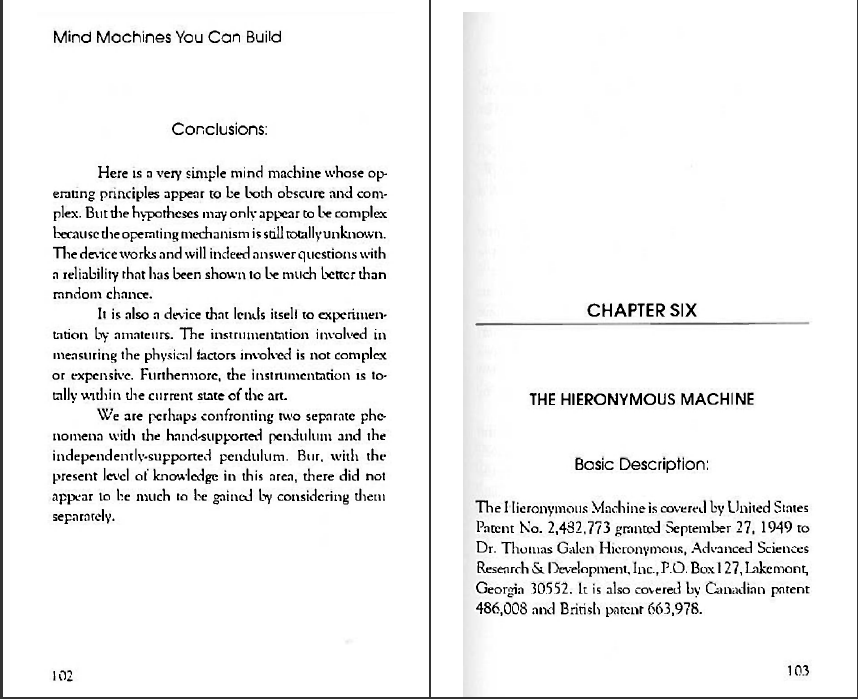
\includegraphics[width=0.6\textwidth]{./chapters/chapter10}
\end{figure}

\lipsum[1]
>>>>>>> merged

\cxset{chapter opening=any}
% Copyright 2006 by Till Tantau
%
% This file may be distributed and/or modified
%
% 1. under the LaTeX Project Public License and/or
% 2. under the GNU Free Documentation License.
%
% See the file doc/generic/pgf/licenses/LICENSE for more details.


\chapter{Matrix Library}

\begin{tikzlibrary}{matrix}
  This library packages defines additional styles and options for
  creating matrices.
\end{tikzlibrary}


\section{Matrices of Nodes}

A \emph{matrix of nodes} is a \tikzname\ matrix in which each cell
contains a node. In this case it is bothersome having to write
|\node{| at the beginning of each cell and |};| at the end of each
cell. The following key simplifies typesetting such matrices.

\begin{key}{/tikz/matrix of nodes}
  Conceptually, this key adds |\node{| at the beginning and |};| at
  the end of each cell and sets the |anchor| of the node to
  |base|. Furthermore, it adds  the option |name| option to each node,
  where the name is set to  \meta{matrix name}|-|\meta{row
    number}|-|\meta{column number}. For  example, if the matrix has
  the name |my matrix|, then the node in  the upper left cell will get
  the name |my matrix-1-1|. 
\begin{codeexample}[]
\begin{tikzpicture}
  \matrix (magic) [matrix of nodes]
  {
    8 & 1 & 6 \\
    3 & 5 & 7 \\
    4 & 9 & 2 \\
  };

  \draw[thick,red,->] (magic-1-1) |- (magic-2-3);
\end{tikzpicture}
\end{codeexample}

  You may wish to add options to certain nodes in the matrix. This can
  be achieved in three ways.
  \begin{enumerate}
  \item You can modify, say, the
    |row 2 column 5| style to pass special options to this particular
    cell.

\begin{codeexample}[]
\begin{tikzpicture}[row 2 column 3/.style=red]
  \matrix [matrix of nodes]
  {
    8 & 1 & 6 \\
    3 & 5 & 7 \\
    4 & 9 & 2 \\
  };
\end{tikzpicture}
\end{codeexample}
    
  \item At the beginning of a cell, you can use a special syntax. If a
    cell starts with a vertical bar, then everything between this bar
    and the next bar is passed on to the |node| command.
{\catcode`\|=12
\begin{codeexample}[]
\begin{tikzpicture}
  \matrix [matrix of nodes]
  {
    8 & 1 &         6 \\
    3 & 5 & |[red]| 7 \\
    4 & 9 &         2 \\
  };
\end{tikzpicture}
\end{codeexample}
}
  You can also use an option like \verb!|[red] (seven)|! to give a
  different name to the node.

  Note that the |&| character also takes an optional argument, which
  is an extra column skip.
{\catcode`\|=12  
\begin{codeexample}[]
\begin{tikzpicture}
  \matrix [matrix of nodes]
  {
    8 &[1cm] 1 &[3mm] |[red]| 6 \\
    3 &      5 &      |[red]| 7 \\
    4 &      9 &              2 \\
  };
\end{tikzpicture}
\end{codeexample}
}
  \item If your cell starts with a |\path| command or any command that
    expands to |\path|, which includes |\draw|, |\node|, |\fill| and
    others, the |\node{| startup code and the |};| code are
    suppressed. This means that for this particular cell you can
    provide a totally different contents.

\begin{codeexample}[]
\begin{tikzpicture}
  \matrix [matrix of nodes]
  {
    8 & 1 & 6 \\
    3 & 5 & \node[red]{7}; \draw(0,0) circle(10pt);\\
    4 & 9 & 2 \\
  };
\end{tikzpicture}
\end{codeexample}
  \end{enumerate}
\end{key}

\begin{key}{/tikz/matrix of math nodes}
  This style is almost the same as the previous style, only |$| is %$
  added at the beginning and at the end of each node, so math mode
  will be switched on in all nodes.
{\catcode`\|=12
\begin{codeexample}[]
\begin{tikzpicture}
  \matrix [matrix of math nodes]
  {
    a_8 & a_1 &         a_6 \\
    a_3 & a_5 & |[red]| a_7 \\
    a_4 & a_9 &         a_2 \\
  };
\end{tikzpicture}
\end{codeexample}
}
\end{key}

\begin{key}{/tikz/nodes in empty cells=\meta{true or false} (default true)}
  When set to |true|, a node (with an empty contents) is put in empty
  cells. Normally, empty cells are just, well, empty. The style can be
  used together with both a |matrix of nodes| and a
  |matrix of math nodes|.
\begin{codeexample}[]
\begin{tikzpicture}
  \matrix [matrix of math nodes,nodes={circle,draw}]
  {
    a_8 &     & a_6 \\
    a_3 &     & a_7 \\
    a_4 & a_9 &     \\
  };
\end{tikzpicture}
\end{codeexample}
\begin{codeexample}[]
\begin{tikzpicture}
  \matrix [matrix of math nodes,nodes={circle,draw},nodes in empty cells]
  {
    a_8 &     & a_6 \\
    a_3 &     & a_7 \\
    a_4 & a_9 &     \\
  };
\end{tikzpicture}
\end{codeexample}
\end{key}


\subsection{End-of-Lines and End-of-Row Characters in Matrices of Nodes}

Special care must be taken about the usage of the |\\| command inside
a matrix of nodes. The reason is that this character is overloaded in
\TeX: On the one hand, it is used to denote the end of a line in
normal text; on the other hand it is used to denote the end of a row
in a matrix. Now, if a matrix contains node which in turn may have
multiple lines, it is unclear which meaning of |\\| should be used.

This problem arises only when you use the |text width| option of
nodes. Suppose you write a line like
\begin{codeexample}[code only]
\matrix [text width=5cm,matrix of nodes]
{
  first row & upper line \\ lower line \\
  second row & hmm \\
};
\end{codeexample}
This leaves \TeX\ trying to riddle out how many rows this matrix
should have. Do you want two rows with the upper right cell containing
a two-line text. Or did you mean a three row matrix with the second
row having only one cell?

Since \TeX\ is not clairvoyant, the following rules are used:
\begin{enumerate}
\item Inside a matrix, the |\\| command, by default, signals the end
  of the row, not the end of a line in a cell.
\item However, there is an exception to this rule: If a cell
  starts with a \TeX-group (this is, with |{|), % }
  then inside this first group the |\\| command retains the meaning of
  ``end of line'' character. Note that this special rule works only
  for the first group in a cell and this group must be at the
  beginning. 
\end{enumerate}

The net effect of these rules is the following: Normally, |\\| is an
end-of-row indicator; if you want to use it as an end-of-line
indicator in a cell, just put the whole cell in curly braces. The
following example illustrates the difference:
\begin{codeexample}[]
\begin{tikzpicture}
  \matrix [matrix of nodes,nodes={text width=16mm,draw}]
  {
    row 1 & upper line \\ lower line \\
    row 2 & hmm \\
  };
\end{tikzpicture}
\end{codeexample}
\begin{codeexample}[]
\begin{tikzpicture}
  \matrix [matrix of nodes,nodes={text width=16mm,draw}]
  {
    row 1 & {upper line \\ lower line} \\
    row 2 & hmm \\
  };
\end{tikzpicture}
\end{codeexample}

Note that this system is not fool-proof. If you write things like
|a&b{c\\d}\\| in a matrix of nodes, an error will result (because the
second cell did not start with a brace, so |\\| retained its normal
meaning and, thus, the second cell contained the text |b{c|, which is
not balanced with respect to the number of braces).

\subsection{Delimiters}

Delimiters are parantheses or braces to the left and right of a
formula or a matrix. The matrix library offers options for adding such
delimiters to a matrix. However, delimiters can actually be added to
any node that has the standard anchors |north|, |south|, |north west|
and so on. In particular, you can add delimiters to any |rectangle|
box. They are implemented by ``measuring the height'' of the node and
then adding a delimiter of the correct size to the left or right using
some after node magic.

\begin{key}{/tikz/left delimiter=\meta{delimiter}}
  This option can be given to a any node that has the standard anchors
  |north|, |south| and so on. The \meta{delimiter} can be any
  delimiter that is acceptable to \TeX's |\left| command.
\begin{codeexample}[]
\begin{tikzpicture}
  \matrix [matrix of math nodes,left delimiter=(,right delimiter=\}]
  {
    a_8 & a_1 & a_6 \\
    a_3 & a_5 & a_7 \\
    a_4 & a_9 & a_2 \\
  };
\end{tikzpicture}
\end{codeexample}

\begin{codeexample}[]
\begin{tikzpicture}
  \node [fill=red!20,left delimiter=(,right delimiter=\}]
    {$\displaystyle\int_0^1 x\,dx$};
\end{tikzpicture}
\end{codeexample}

  \begin{stylekey}{/tikz/every delimiter (initially \normalfont empyt)}
    This style is executed for every delimiter. You can use it to shift
    or color delimiters or do whatever.
  \end{stylekey}

  \begin{stylekey}{/tikz/every left delimiter (initially \normalfont empty)}
    This style is additionally executed for every left delimiter.
\begin{codeexample}[]
\begin{tikzpicture}
  [every left delimiter/.style={red,xshift=1ex},
   every right delimiter/.style={xshift=-1ex}]
  \matrix [matrix of math nodes,left delimiter=(,right delimiter=\}]
  {
    a_8 & a_1 & a_6 \\
    a_3 & a_5 & a_7 \\
    a_4 & a_9 & a_2 \\
  };
\end{tikzpicture}
\end{codeexample}
  \end{stylekey}
\end{key}

\begin{key}{/tikz/right delimiter=\meta{delimiter}}
  Works as above.
  \begin{stylekey}{/tikz/every right delimiter (initially \normalfont empty)}
    Works as above.
  \end{stylekey}
\end{key}


\begin{key}{/tikz/above delimiter=\meta{delimiter}}
  This option allows you to add a delimiter above the node. It is
  implementing by rotating a left delimiter.
\begin{codeexample}[]
\begin{tikzpicture}
  \matrix [matrix of math nodes,%
           left delimiter=\|,right delimiter=\rmoustache,%
           above delimiter=(,below delimiter=\}]
  {
    a_8 & a_1 & a_6 \\
    a_3 & a_5 & a_7 \\
    a_4 & a_9 & a_2 \\
  };
\end{tikzpicture}
\end{codeexample}

  \begin{stylekey}{/tikz/every above delimiter (initially \normalfont empty)}
    Works as above.
  \end{stylekey}
\end{key}

\begin{key}{/tikz/below delimiter=\meta{delimiter}}
  Works as above.
  \begin{stylekey}{/tikz/every below delimiter (initially \normalfont empty)}
    Works as above.
  \end{stylekey}
\end{key}



%%% Local Variables: 
%%% mode: latex
%%% TeX-master: "pgfmanual-pdftex-version"
%%% End: 


\chapter{Plotting
}
\pgfplotsset{
tick label style={font=\small},
label style={font={\small\sffamily}},
legend style={font={\footnotesize\sffamily}}
}
\begin{codeexample}[]
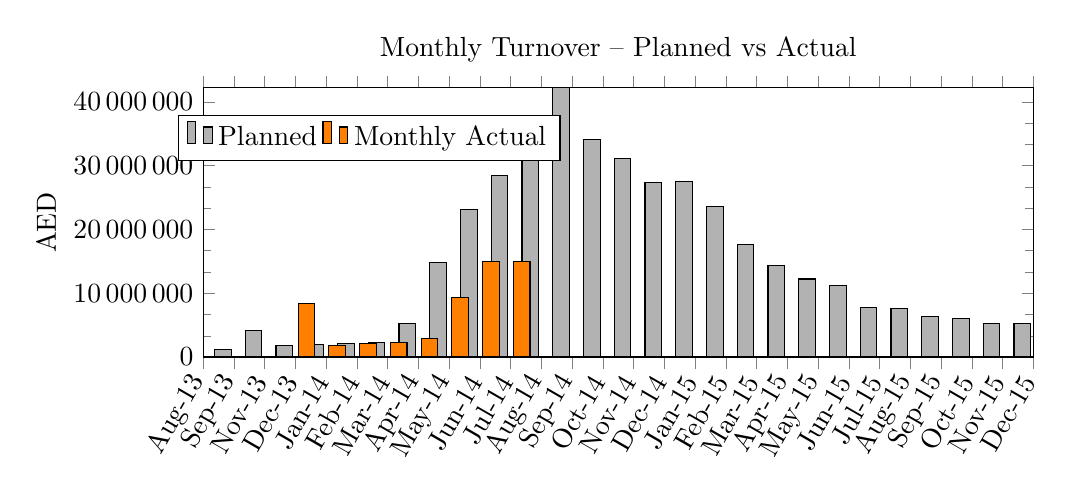
\begin{tikzpicture}
\begin{axis}[
   title={Monthly Turnover -- Planned vs Actual},
   width=1\textwidth,
   height=5cm,
   bar width=6pt,
   minor y tick num=2,
   xmajorgrids = false,
   yminorgrids=false,
   ylabel shift= -.5,
	ybar,
	enlargelimits=0.0,
	legend style={at={(0.2,0.9)},anchor=north,
	anchor=north,legend columns=-1},
	ylabel={AED},
   ytick = {0,10000000,20000000,30000000,40000000},
   scaled ticks = false,
   y tick label style={
        /pgf/number format/.cd,
            1000 sep={\,},
            fixed,
            fixed zerofill,
            precision=0,
                   /tikz/.cd
    },
	symbolic x coords={Aug-13,Sep-13,Nov-13,Dec-13,
                      Jan-14,Feb-14,Mar-14,Apr-14,
                      May-14,Jun-14,Jul-14,Aug-14,
                      Sep-14,Oct-14,Nov-14,Dec-14,
                      Jan-15,Feb-15,Mar-15,Apr-15,
                      May-15,Jun-15,Jul-15,Aug-15,
                      Sep-15,Oct-15,Nov-15,Dec-15},
	xtick = data,
   x tick label style={rotate=60,anchor=east},
   ] 
	%nodes near coords,
	nodes near coords align={vertical},
]
\addplot[fill=black!30] coordinates {(Aug-13, 29275) 
                      (Sep-13, 1118506) 
                      (Nov-13, 4118404) 
                      (Dec-13, 1744492)
                      (Jan-14, 1929106)
                      (Feb-14, 2071614)
                      (Mar-14, 2291612)
                      (Apr-14, 5280597)
                      (May-14, 14826470)
                      (Jun-14, 23178070)
                      (Jul-14, 28436550)
                      (Aug-14, 34928860)
                      (Sep-14, 42203710)
                      (Oct-14, 34092590)
                      (Nov-14, 31064640)
                      (Dec-14, 27368860)
                      (Jan-15, 27539670)
                      (Feb-15, 23631860)
                      (Mar-15, 17713270)
                      (Apr-15, 14334710)
                      (May-15, 12238960)
                      (Jun-15, 11169200)
                      (Jul-15, 7822311)
                      (Aug-15, 7654239)
                      (Sep-15, 6298405)
                      (Oct-15,6069190)
                      (Nov-15,5292039)
                      (Dec-15,5310467) 
         };
\addplot[fill=orange] coordinates {(Aug-13, 0) 
                      (Sep-13, 0) 
                      (Nov-13, 0)
                      (Dec-13, 8330874)
                      (Jan-14, 1835372) 
                      (Feb-14, 2116680)
                      (Mar-14, 2284853)
                      (Apr-14, 2860646)
                      (May-14, 9301770) 
                      (Jun-14, 15000000)
                      (Jul-14, 15000000)
};

\legend{Planned, Monthly Actual}
\end{axis}
\end{tikzpicture}
\label{barchart}
\end{codeexample}

\kant[1]
\end{document}

\endinput
%%
%% End of file `test-spacing.tex'.
